\documentclass[journal,12pt,twocolumn]{IEEEtran}

\usepackage{setspace}
\usepackage{gensymb}

\singlespacing


\usepackage[cmex10]{amsmath}

\usepackage{amsthm}

\usepackage{mathrsfs}
\usepackage{txfonts}
\usepackage{stfloats}
\usepackage{bm}
\usepackage{cite}
\usepackage{cases}
\usepackage{subfig}

\usepackage{longtable}
\usepackage{multirow}

\usepackage{enumitem}
\usepackage{mathtools}
\usepackage{steinmetz}
\usepackage{tikz}
\usepackage{circuitikz}
\usepackage{verbatim}
\usepackage{tfrupee}
\usepackage[breaklinks=true]{hyperref}
\usepackage{graphicx}
\usepackage{tkz-euclide}

\usetikzlibrary{calc,math}
\usepackage{listings}
    \usepackage{color}                                            %%
    \usepackage{array}                                            %%
    \usepackage{longtable}                                        %%
    \usepackage{calc}                                             %%
    \usepackage{multirow}                                         %%
    \usepackage{hhline}                                           %%
    \usepackage{ifthen}                                           %%
    \usepackage{lscape}     
\usepackage{multicol}
\usepackage{chngcntr}

\DeclareMathOperator*{\Res}{Res}

\renewcommand\thesection{\arabic{section}}
\renewcommand\thesubsection{\thesection.\arabic{subsection}}
\renewcommand\thesubsubsection{\thesubsection.\arabic{subsubsection}}

\renewcommand\thesectiondis{\arabic{section}}
\renewcommand\thesubsectiondis{\thesectiondis.\arabic{subsection}}
\renewcommand\thesubsubsectiondis{\thesubsectiondis.\arabic{subsubsection}}


\hyphenation{op-tical net-works semi-conduc-tor}
\def\inputGnumericTable{}                                 %%

\lstset{
%language=C,
frame=single, 
breaklines=true,
columns=fullflexible
}
\begin{document}


\newtheorem{theorem}{Theorem}[section]
\newtheorem{problem}{Problem}
\newtheorem{proposition}{Proposition}[section]
\newtheorem{lemma}{Lemma}[section]
\newtheorem{corollary}[theorem]{Corollary}
\newtheorem{example}{Example}[section]
\newtheorem{definition}[problem]{Definition}

\newcommand{\BEQA}{\begin{eqnarray}}
\newcommand{\EEQA}{\end{eqnarray}}
\newcommand{\define}{\stackrel{\triangle}{=}}
\bibliographystyle{IEEEtran}
\providecommand{\mbf}{\mathbf}
\providecommand{\pr}[1]{\ensuremath{\Pr\left(#1\right)}}
\providecommand{\qfunc}[1]{\ensuremath{Q\left(#1\right)}}
\providecommand{\sbrak}[1]{\ensuremath{{}\left[#1\right]}}
\providecommand{\lsbrak}[1]{\ensuremath{{}\left[#1\right.}}
\providecommand{\rsbrak}[1]{\ensuremath{{}\left.#1\right]}}
\providecommand{\brak}[1]{\ensuremath{\left(#1\right)}}
\providecommand{\lbrak}[1]{\ensuremath{\left(#1\right.}}
\providecommand{\rbrak}[1]{\ensuremath{\left.#1\right)}}
\providecommand{\cbrak}[1]{\ensuremath{\left\{#1\right\}}}
\providecommand{\lcbrak}[1]{\ensuremath{\left\{#1\right.}}
\providecommand{\rcbrak}[1]{\ensuremath{\left.#1\right\}}}
\theoremstyle{remark}
\newtheorem{rem}{Remark}
\newcommand{\sgn}{\mathop{\mathrm{sgn}}}
\providecommand{\abs}[1]{\left\vert#1\right\vert}
\providecommand{\res}[1]{\Res\displaylimits_{#1}} 
\providecommand{\norm}[1]{\left\lVert#1\right\rVert}
%\providecommand{\norm}[1]{\lVert#1\rVert}
\providecommand{\mtx}[1]{\mathbf{#1}}
\providecommand{\mean}[1]{E\left[ #1 \right]}
\providecommand{\fourier}{\overset{\mathcal{F}}{ \rightleftharpoons}}
%\providecommand{\hilbert}{\overset{\mathcal{H}}{ \rightleftharpoons}}
\providecommand{\system}{\overset{\mathcal{H}}{ \longleftrightarrow}}
	%\newcommand{\solution}[2]{\textbf{Solution:}{#1}}
\newcommand{\solution}{\noindent \textbf{Solution: }}
\newcommand{\cosec}{\,\text{cosec}\,}
\providecommand{\dec}[2]{\ensuremath{\overset{#1}{\underset{#2}{\gtrless}}}}
\newcommand{\myvec}[1]{\ensuremath{\begin{pmatrix}#1\end{pmatrix}}}
\newcommand{\mydet}[1]{\ensuremath{\begin{vmatrix}#1\end{vmatrix}}}
\numberwithin{equation}{subsection}
\makeatletter
\@addtoreset{figure}{problem}
\makeatother
\let\StandardTheFigure\thefigure
\let\vec\mathbf
\renewcommand{\thefigure}{\theproblem}
\def\putbox#1#2#3{\makebox[0in][l]{\makebox[#1][l]{}\raisebox{\baselineskip}[0in][0in]{\raisebox{#2}[0in][0in]{#3}}}}
     \def\rightbox#1{\makebox[0in][r]{#1}}
     \def\centbox#1{\makebox[0in]{#1}}
     \def\topbox#1{\raisebox{-\baselineskip}[0in][0in]{#1}}
     \def\midbox#1{\raisebox{-0.5\baselineskip}[0in][0in]{#1}}
\vspace{3cm}
\title{Assignment 5}
\author{R.OOHA}
\maketitle
\newpage
\bigskip
\renewcommand{\thefigure}{\theenumi}
\renewcommand{\thetable}{\theenumi}
Download all python codes from 
\begin{lstlisting}p
https://github.com/ooharapolu/ASSIGNMNT5/Assignment5.py
\end{lstlisting}
%
and latex-tikz codes from 
%
\begin{lstlisting}
https://github.com/ooharapolu/ASSIGNMNT5/main.tex
\end{lstlisting}
%
\section{Question No.2.158}
Find the area lying in the first quadrant and by the circle $\vec{x}^T\vec{x}=4$ and the lines $\vec{x}=0$ and $\vec{x}=2$ .
%
\section{Solution}
The given lines of the vector form is,
\begin{align}
\myvec{1 & 0}\vec{x}=0
\\
\myvec{1 & 0}\vec{x}=2
\end{align}
The general equation of the circle is,
\begin{align}
\vec{x}^T\vec{x} + 2\vec{u}^T\vec{x} + f = 0  
\\
\norm{\vec{x}}^2 + 2\vec{u_1}^T\vec{x} + f_1 = 0
\\
\vec{x}^T\vec{x}- 4 = 0
\\
\vec{u_1} = \myvec{0 \\ 0},f_1=-4
\end{align}
To find points A,x and B
\\
The parametric form of x-axis is,
\begin{align}
\vec{B}=\vec{q}+\lambda \vec{m}\\
=\myvec{0\\0}+\lambda \myvec{1\\0} \label{2.0.8}
\end{align}
From the intersection of circle and line,the value of $\lambda$ can be found by,
\begin{align}
\vec{\lambda^2}=\frac{{{-f_1}-\norm{\vec{q}}^2 }}{{\norm {\vec{m}}^2}}=\frac{{{4}-{0} }}{{ {1 }}}=4
\\
\implies \vec{\lambda}=\pm{2} \label{2.0.10}
\end{align}
 point of intersection sub equation \eqref{2.0.10} in \eqref{2.0.8}
\\
Put, $\vec{\lambda}= 2$
\begin{align}
\vec{B}=\myvec{0\\0}+2\myvec{1\\ 0}=\myvec{2 \\ 0}
\\ 
\implies\vec{B}=\myvec{2\\0}
\end{align}
and, $\vec{\lambda}=-2$
\begin{align}
\vec{B}=\myvec{0 \\0}-2\myvec{1\\0}=\myvec{-2 \\ 0}
\\ 
\implies\vec{B}=\myvec{-2\\ 0}
\end{align}
As given in question as first quadrant
\begin{align}
\implies \vec{B}=\myvec{2\\0}   
\end{align}
The parametric form of y-axis is,
\begin{align}
\vec{x}=\vec{q}+\lambda \vec{m}\\
=\myvec{0\\0}+\lambda \myvec{0\\1} \label{2.0.17}
\end{align}
From the intersection of circle and line,the value of $\lambda$ can be found by,
\begin{align}
\vec{\lambda^2}=\frac{{{-f_1}-\norm{\vec{q}}^2 }}{{\norm {\vec{m}}^2}}=\frac{{{4}-{0} }}{{ {1 }}}=4
\\
\implies \vec{\lambda}=\pm{2} \label{2.0.19}
\end{align}
 Point of intersection
Sub equation \eqref{2.0.19} in \eqref{2.0.17}
\\
Put, $\vec{\lambda}= 2$
\begin{align}
\vec{x}=\myvec{0\\0}+2\myvec{0\\ 1}=\myvec{0 \\ 2}
\\ 
\implies\vec{x}=\myvec{0\\2}
\end{align}
and, $\vec{\lambda}=-2$
\begin{align}
\vec{x}=\myvec{0 \\0}-2\myvec{0\\1}=\myvec{0 \\ -2}
\\ 
\implies\vec{x}=\myvec{0\\ -2}
\end{align}
As given in question as first quadrant
\begin{align}
\implies \vec{x}=\myvec{0 \\ 2}   
\end{align}
Similarly,to find point A ,The parametric form of the line is ,
\begin{align}
 \vec{A}=\vec{q}+\lambda \vec{m}\\ =\myvec{2\\0}+\lambda \myvec{0\\1} \label{2.0.26}
\end{align}
\begin{align}
 \vec{\lambda^2}=\frac{{{-f_1}-\norm{\vec{q}}^2}}{{\norm{\vec{m}}^2}}\\=\frac{{{4}-{4}}}{{{1}}}=0
 \\
\implies \lambda=0 \label{2.0.29}
\end{align}
Sub \eqref{2.0.29} in \eqref{2.0.26}
\begin{align}
 \vec{A}=\myvec{2 \\0}+0\myvec{0\\1}=\myvec{2\\0}
 \\
 \implies \vec{A}=\myvec{2 \\ 0}
\end{align}
The equation of a circle can be expressed as,
\begin{align}
\vec{x}^T\vec{x} - 2\vec{u}^T\vec{x} + f= 0\label{2.0.32}
\end{align}
comparing equation \eqref{2.0.32} with the circle equation given,
\begin{align}
\vec{x}^T\vec{x} = 4
\end{align}
\begin{align}
\implies \vec{u}=\myvec{0\\0},f = -4
\\
\implies \vec{r}=\sqrt{\vec{u}^T\vec{x}-{f}}=\sqrt{{4}}
\\
\implies \vec{r} &=2 \label{2.0.36}
\end{align}
Using equation $\eqref{2.0.36}$ and,the area of the sector is obtained as,
\begin{align}
 \implies  \frac{\theta}{360^{\degree}}\pi\vec{r^2}=\frac{90^{\degree}}{360^{\degree}}\pi\myvec{2}^2=\pi
\end{align}
Plot of the given -
\numberwithin{figure}{section}
\begin{figure}[!ht]
\centering
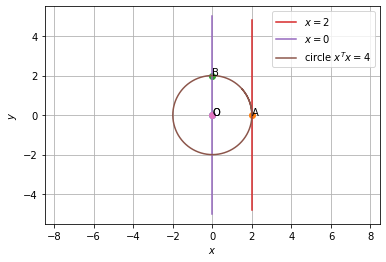
\includegraphics[width=\columnwidth]{Figure 5.png}
\caption{The Circle of the lines }
\label{fig:The circle of the lines}	\end{figure}
\end{document}